% !TEX encoding = UTF-8
\documentclass[UTF8]{ctexart}

\usepackage[utf8]{inputenc}
\usepackage{graphicx}
\usepackage{geometry}
\geometry{a4paper}
\geometry{left=2.5cm,right=2.5cm,top=2.8cm,bottom=1.3cm}

\usepackage{booktabs}
\usepackage{array}
\usepackage{paralist}
\usepackage{verbatim}
\usepackage{subfig}
\usepackage{amsmath}
\usepackage{mathtools}
\usepackage{listings}
\usepackage[table]{xcolor}
\usepackage{lastpage}
\usepackage{url}

% Using hyperref for improved ref character
\usepackage[colorlinks,linkcolor=black,anchorcolor=black,
citecolor=black,CJKbookmarks=True]{hyperref}

% For picture drawing
\usepackage[all]{xy}

% For code inserting. Set features.
\lstset{
alsolanguage=matlab,
tabsize=4,
keepspaces=true,
numbers=left,
numberstyle=\tiny,
keywordstyle=\color{blue!70} \bfseries,
commentstyle=\color{red!50!green!50!blue!50},
frame=shadowbox,
breaklines,
showspaces=false,
showstringspaces=false,
showtabs=false,
rulesepcolor=\color{red!20!green!20!blue!20},
extendedchars=false,
escapeinside=``
}

% Set the font of page header
\usepackage{fancyhdr}
\pagestyle{fancy}
\lhead{传感器特性实验报告}
\chead{}
\rhead{Page \thepage/\pageref{LastPage}}
\cfoot{}
\rfoot{}
\lfoot{}

\usepackage{sectsty}

\usepackage[nottoc]{tocbibind}
\usepackage[titles,subfigure]{tocloft}
\renewcommand{\cftsecfont}{\rmfamily\mdseries\upshape}
\renewcommand{\cftsecpagefont}{\rmfamily\mdseries\upshape}

% Set number of ref to be relevent to section number
\renewcommand{\theequation}{\arabic{section}.\arabic{equation}}
\renewcommand{\thefigure}{\arabic{section}-\arabic{figure}}
\renewcommand{\thetable}{\arabic{section}-\arabic{table}}
\makeatletter
\@addtoreset{equation}{section}
\@addtoreset{figure}{section}
\@addtoreset{table}{section}
\makeatother

% Set the font of the reference
\bibliographystyle{unsrt}

% Define user\rq{}s color
\usepackage{colortbl}
\definecolor{lightgray}{gray}{.9}
\definecolor{thickgray}{gray}{.6}

\usepackage{multirow}

% 首行缩进
\usepackage{indentfirst}

% Set section numbering
\CTEXsetup[number={}]{part}
\renewcommand{\thepart}{}
\usepackage{titlesec}
\titleformat{\part}[block]{\color{blue}\huge\bfseries\filcenter}{}{1em}{}

%\usepackage{ulem}
%\usepackage{indentfirst}
%\setlength\textwidth{300.0pt}
%

% 重定义字体命令
\newcommand{\song}{\CJKfamily{song}}    % 宋体   (Windows自带simsun.ttf)
\newcommand{\fs}{\CJKfamily{fs}}        % 仿宋体 (华天字库htfs.ttf)
\newcommand{\kai}{\CJKfamily{kai}}      % 楷体   (华天字库htkai.ttf)
\newcommand{\hei}{\CJKfamily{hei}}      % 黑体   (Windows自带simhei.ttf)
\newcommand{\li}{\CJKfamily{li}}        % 隶书   (Windows自带simli.ttf)
\newcommand{\you}{\CJKfamily{you}}      % 幼圆体 (Windows自带simyou.ttf)
%%%  以上六种字体均为标准 GBK 字体, 包括 GBK 繁体字和一些不常用字, 推荐!!!

\newcommand{\xs}{\CJKfamily{xs}}
\newcommand{\shu}{\CJKfamily{shu}}      % 舒体   (方正字库fzstk.ttf)
%  \newcommand{\yourcommand}[参数个数]{内容}   [参数个数]这个是可选的。
%  例如  \newcommand{\you}{\CJKfamily{you}}  用\you 来代替 \CJKfamily{you} ,少输入很多字哦。
%字号设置
\newcommand{\chuhao}{\fontsize{42pt}{\baselineskip}\selectfont}
\newcommand{\xiaochuhao}{\fontsize{36pt}{\baselineskip}\selectfont}
\newcommand{\yihao}{\fontsize{28pt}{\baselineskip}\selectfont}
\newcommand{\xiaoyihao}{\fontsize{24pt}{\baselineskip}\selectfont}
\newcommand{\erhao}{\fontsize{21pt}{\baselineskip}\selectfont}
\newcommand{\xiaoerhao}{\fontsize{18pt}{\baselineskip}\selectfont}
\newcommand{\sanhao}{\fontsize{15.75pt}{\baselineskip}\selectfont}
\newcommand{\sihao}{\fontsize{14pt}{\baselineskip}\selectfont}
\newcommand{\xiaosihao}{\fontsize{12pt}{\baselineskip}\selectfont}
\newcommand{\wuhao}{\fontsize{10.5pt}{\baselineskip}\selectfont}
\newcommand{\xiaowuhao}{\fontsize{9pt}{\baselineskip}\selectfont}
\newcommand{\liuhao}{\fontsize{7.875pt}{\baselineskip}\selectfont}
\newcommand{\qihao}{\fontsize{5.25pt}{\baselineskip}\selectfont}
% \baselineskip | distance from bottom of one line of a paragraph to bottom of the next line.  基本行距
%  只有使用\selectfont命令之后,\fontzize{}{}的设置才能生效
%  可以用数字表示{11pt}:单倍行距

\begin{document}
%%%%%%%%%%%%%%%%%%%%%%%%%%%%封面与目录%%%%%%%%%%%%%%%%%%%%%%%%%%%%%%
\begin{titlepage}
\begin{center}
% Upper part of the page

\includegraphics[width=0.25\textwidth]{resource/logo.jpg}\\[1cm]
\textsc{\LARGE Department of Automation}\\[1.5cm]
\fs{\Large 检测原理系列实验}\\[0.5cm]
% Title
\hrulefill
\\[0.8cm]{\centering \huge \hei 传感器特性实验报告}\\[0.4cm]
\hrulefill
\\[4cm]

% Author and supervisor
\begin{tabbing}       %tabbing  列表

 \hspace*{5cm} \= \hspace{2.6cm} \= \kill
 % \=     in tabbing environment, sets a tab stop
 % \kill  in a\tabbing environment, deletes previous line so tabs can be set without outputting text.
 % \>     in tabbing environment is a forward tab.

\>{\fs\sihao\textbf {班\hspace{1cm}级 \ \ :}}\>  {\centering\fs\sihao\textbf{~~~~~~~~~~~自~~3~2}} \\
\\
\>{\fs\sihao\textbf {姓\hspace{1cm}名 \ \ :}}\>  {\centering\fs\sihao\textbf{~陈~昊~楠~(2013011449)}}\\
\\
\>{\fs\sihao\textbf {同\hspace{0.2cm}组\hspace{0.3cm}人 \ \ :}}\>  {\centering\fs\sihao\textbf{~陈~炜~祥~(2013011456)}}\\
\\
\>{\fs\sihao\textbf {指导教师 \ \ :}}\>  {\centering\fs\sihao\textbf{~~~~~~~~~~~陆~~~~~耿}} \\

\end{tabbing}
\vfill
{\large \today}
\end{center}
\end{titlepage}

\tableofcontents
\clearpage

%%%%%%%%%%%%%%%%%%%%%%%%%%正文部分%%%%%%%%%%%%%%%%%%%%%%%%%%%%%%%%%%
\part{AS-i总线技术(V3.0)特性研究}
\section{AS-i总线原理与特点}
\subsection{AS-i总线概述}
AS-i是“执行器-传感器-接口”的英文缩写(Actuator Sensor- interface)。它是一种用来在控制器(主站)和传感器/执行器(从站)之间双向交换信息、主从结构的总线网络,它属于现场总线下面底层的监控网络系统。\\
AS-i主站是AS-i总线系统的核心,它由AS-i主机和控制器(如PC和PLC等)组成。向上通过主站中的网关可以和多种现场总线(如PROFIBUS,FF,CANBUS等)进行连接,向下可以挂接一批AS-i从站,主站将按照AS-i通信协议与各个从站之间进行数据交换。\\
AS-i从站一般可分为两种类型,一种是智能型开关装置,它本身就带有从机专用芯片和配套电路,形成一体化从站,这种智能型传感器/执行器可以直接和AS-i总线连接。第二种是专门设计的AS-i 连接模块,在这种模块中带有从机专用芯片和配套电路,它除了具有通信接口外还带有I/O接口,这些I/O接口可以和普通的传感器/执行器相连接构成分离型从站。\\
AS-i系统主站和从站之间的通信采用非屏蔽、非绞接的两芯电缆。其中一种是普通的圆柱形电缆,另一种是专用的扁平电缆,由于扁平电缆采用一种特殊的穿刺安装方式把线压在连接件上,所以安装拆卸即简单又可靠。在两芯电缆上除传输信号外还通过网络向主站和从站提供电源。
\subsection{AS-i技术规范V3.0特点}
2006年AS-i国际协会发布了最新的AS-i技术规范V3.0,它比原有的V2.1版本有了更大的改进,并完全兼容以前版本的技术内容,最大的改进有以下两点:
\begin{enumerate}
\item 增加了AS-i安全系统元件的规范。
\item 增加了新的AS-i主站和从站规范以及组合处理类型(CTT,Combined Transaction Type)的定义。
\end{enumerate}
在自动化生产现场,不同的客户有不同的需求,特别是对于从站的性能、连接、安装都有不同的要求。在新的V3.0规范中,增加了很多新的从站规范,这也使生产商可以给客户提供更加多样化的产品。随着自动化产品在监控系统中的广泛应用,安全概念的不断变革和安全技术的不断更新,作为现场最底层的AS-i总线系统也在新的V3.0规范中增加了相关安全系统产品的规范。组合处理类型(CTT)的定义为AS-i系统的通讯增加了新的功能,包括对模拟量模块和安全输入/输出模块的通讯支持。
\section{实验内容与分析}
\subsection{编址}
按照实验指导书进行操作,找到了各个网关对应传感器的位置,并学习了使用手持编程器编址和网关编址的方法。最终确定的编址如表\ref{tab:aa}。

\begin{table}[htbp]
\centering
\begin{tabular}{|c|c|c|}
	\hline
	从站类型 & 从站名称 & 地址 \\
	\hline
	开关量 & 控制箱型 4 入/4 出模块 & 2A \\
	开关量 & 现场型 4 入/4 出模块 & 4A \\
	开关量 & 现场紧凑型 2 输入模块 & 5A \\
	模拟量 & 现场型 2 输入模块 & 3 \\
	模拟量 & 控制箱型 2 输出模块 & 1 \\
	\hline
\end{tabular}
\caption{AS-i从站地址}
\label{tab:aa}
\end{table}

\subsection{错误诊断}
实验现象如下:
\paragraph{一个AS-i从站丢失}
\begin{enumerate}
\item 拔出现场型4入/4出模块,网关LCD显示器显示 {\ttfamily Missing 4A},Config err红灯亮;将现场型4入/4出模块重新接入系统,网关红灯灭,系统恢复正常。这是因为该模块地址没有变,只是拔下模块,系统在轮询到该地址时将不会得到输入信号,因此显示丢失。重新接入后又能询问到信号,因此恢复正常。
\item 将现场型2输入模拟量模块的紧固螺钉拧松,使网关LCD显示器显示 {\ttfamily Missing 3},Config err红灯亮。将其重新编址为6,再次接入没有恢复正常(此时总线系统处于运行模式),进退一次配置模式,则恢复正常且模块被编址为6。
\item 将现场型2输入模拟量模块的紧固螺钉拧松,使网关LCD显示器显示 {\ttfamily Missing 3},Config err红灯亮。将其重新编址为0,再次接入则恢复正常,模块地址仍为6。
\end{enumerate}
\paragraph{一个AS-i从站未配置}
\begin{enumerate}
\item 将现场型4入/4出模块的电源插头(黑色)拧下,即卸掉1个从站。将网关置于配置模式,网关LCD显示器将循环显示系统中的4个从站地址。然后保存当前配置并将网关置于运行模式,AS-i系统运行正常。
\item 将现场型4入/4出模块重新接入系统,Config err红灯亮,模块的 {\ttfamily Fault}红灯亮,网关LCD显示器显示 {\ttfamily Unknown 4A}。重新进退一次配置模式,则系统又恢复正常。因为配置模式中可以重新设定所有的地址,之前地址没有冲突,因此是可以重新设定的。
\end{enumerate}
\paragraph{两个AS-i从站地址相同}
\begin{enumerate}
\item 将网关置于配置模式,用手持编程器为控制箱型2输出模拟量模块和现场型2输入模拟量模块的地址配置为相同地址,保存当前配置并将网关置于运行模式,网关的 Config err 红灯亮,显示 {\ttfamily Missing 1} 和 {\ttfamily Duplicate 3}。
\item 重新置网关于配置模式,用手持编程器为控制箱型2输出模拟量模块和现场型2输入模拟量模块的地址重新配置为不同的地址,网关LCD显示器将循环显示系统中的5个从站地址,保存当前配置并将网关置于运行模式,AS-i系统恢复正常。
\end{enumerate}

\subsection{数据表示方法}
AS-i从站的I/O模块都可以下接一些传感器。本实验分别对5个AS-i从站(即5种不同的I/O模块),以及它们各自接入的传感器或执行器的种类和占用的数据位进行考察。确认数据位可以通过每个I/O模块面板指示灯,或通过网关高级显示模式。在AS-i控制工具软件中也可以看到这种变化,参见下一节的实验。\\
实验现象见表\ref{tab:dr}。其中超声波接在了控制箱型 2 输出模块的1通道。
\begin{table}[htbp]
\centering
\begin{tabular}{|c|c|c|c|}
	\hline
	传感器 & 所接从站地址 & 通过I/O模块 & 通过显示模式 \\
	\hline
	电容式 & 2A & 4号黄灯亮 & 0000变为1000 \\
	反射板型光电 & 4A & IN1灭 & 0001变为0000 \\
	电磁式 & 5A & I2亮 & 0001变为0011 \\
	色标对比 & 5A & I1灭 & 0001变为0000 \\
	倾角 & 1 & & 滚动条跟踪变化,0和1都变\\
	超声波 & 1 & & 滚动条跟踪变化,只有1变 \\
	\hline
\end{tabular}
\caption{AS-i系统数据表示方法实验现象}
\label{tab:dr}
\end{table}

\subsection{AS-i控制工具软件使用}
按照实验指导书进行软件的配置。
\paragraph{编址}
若在线修改从站系统的地址,观察到软件界面右下角出现 {\ttfamily Configuration error},面板红灯亮。
\paragraph{数据表示方法}
点击控制箱型 4 入/4 出模块(对应电容传感器)地址位,在 {\ttfamily Slave Configurtion Address} 的 {\ttfamily Data and parameter} 菜单项中观察,激活电容传感器,对应Input 3 打勾。用鼠标分别点中这个模块输出Outputs\quad 0,1,2,3,模块面板上OUT\quad 1,2,3,4的黄灯亮。

\subsection{AS-i输出模块的看门狗功能}
\paragraph{看门狗功能开启}
中断通信,模块的FAULT指示灯全亮,且输出黄灯灭,网关LED灯灭。重新将通信置于正常,FAULT指示灯灭,输出黄灯和网关LED又按原来的方式亮。
\paragraph{看门狗功能取消}
中断通信,模块的FAULT指示灯全亮,但输出黄灯不灭,网关LED灯也不灭灭。重新将通信置于正常,FAULT指示灯灭。

\subsection{色标、超声波和倾角传感器的调节方法}
\paragraph{色标传感器} 按指导书调节即可。
\paragraph{超声波传感器} 按指导书设定传感器的A1,A2工作点,在网关LCD显示屏进入 {\ttfamily Analog Input} 跟踪传感器输出,记录目标板与传感器间距和输入通道示数的关系如表\ref{tab:dc}。关系曲线如图\ref{fig:dcr}。

\begin{table}[htbp]
\centering
\begin{tabular}{|c|ccccc|}
	\hline
	目标板与传感器间距(cm) & 5 & 10 & 15 & 20 & 25 \\
	\hline
	输入通道示数 & 3994 & 7643 & 12302 & 16523 & 19977 \\
	\hline
\end{tabular}
\caption{超声传感器距离与输出关系}
\label{tab:dc}
\end{table}

\begin{figure}[htbp]
\centering
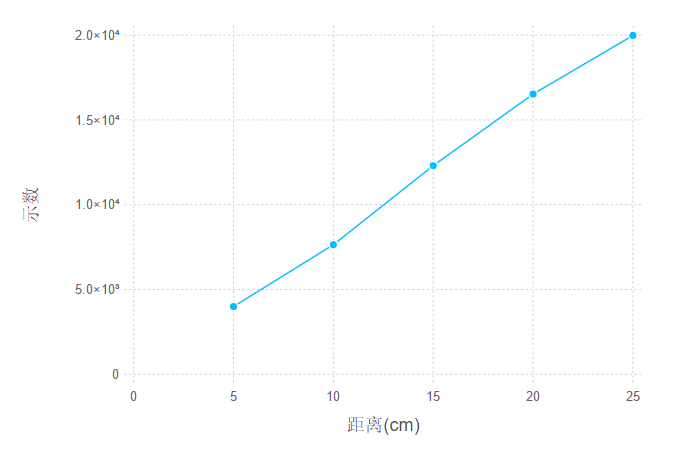
\includegraphics[width=11cm]{resource/dcr.png}
\caption{超声传感器距离示数曲线}
\label{fig:dcr}
\end{figure}

\paragraph{倾角传感器} 按指导书设定传感器的x,y轴输出模式,在网关LCD显示屏进入 {\ttfamily Analog Input} 跟踪传感器输出,记录目标板与传感器x,y方向倾角和输入通道示数的关系如表\ref{tab:dq}。关系曲线如图\ref{fig:dqr}。

\begin{table}[htbp]
\centering
\begin{tabular}{|c|c|ccccccc|}
	\hline
	\multirow{2}*{x方向} & 倾角 & $0^{\circ}$ & $15^{\circ}$ & $30^{\circ}$ &
		$45^{\circ}$ & $60^{\circ}$ & $75^{\circ}$ & $90^{\circ}$ \\
	\cline{2-9}
	& 输入通道示数 & 4139 & 4670 & 6146 & 7026 & 8253 & 9371 & 11431 \\
	\hline
	\multirow{2}*{y方向} & 倾角 & $0^{\circ}$ & $15^{\circ}$ & $30^{\circ}$ &
		$45^{\circ}$ & $60^{\circ}$ & $75^{\circ}$ & $90^{\circ}$ \\
	\cline{2-9}
	& 输入通道示数 & 4234 & 4767 & 5318 & 5982 & 6731 & 7106 & 8381 \\
	\hline
\end{tabular}
\caption{倾角传感器x,y方向倾角与输出关系}
\label{tab:dq}
\end{table}

\begin{figure}[htbp]
\centering
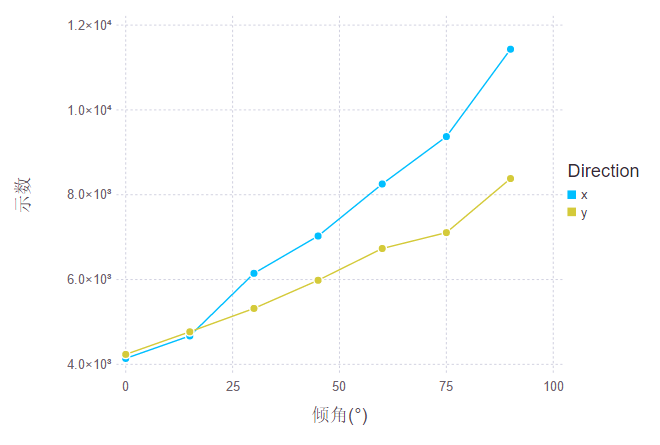
\includegraphics[width=11cm]{resource/dqr.png}
\caption{倾角传感器距离示数曲线}
\label{fig:dqr}
\end{figure}

\section{思考题}
\begin{enumerate}
\item 利用网关给从站编址,网关处于配置模式和运行模式方法一样吗?为什么?\\
不一样。处于配置模式时,对地址进行的修改在退出配置模式即可保存;处于运行模式时,对地址进行修改会亮红灯报错,只有先进入、再退出配置模式才能消除错误,保存更改。
\item 0地址的作用?自动赋值功能需满足那些条件?\\
从错误诊断部分的实验结果来看,0地址表示自动分配地址。自动赋值功能需要拔下之前地址分配没有错误,且地址没有在配置模式中重新设定过,网关才能确定需要自动为其分配的地址值。
\item 输出模块“看门狗”功能的作用是什么?\\
看门狗为整个系统的中保护机制,当通信断开时候,会限制输出为低电平, 从而保护电路输出及工作人员的安全。

\end{enumerate}
\part{实现PLC控制器对其外围I/O设备的控制}
\section{实验原理}
\subsection{PLC控制器功能}
\
\subsection{编程方法}
\section{实验内容}
\subsection{模块地址与端口}
将网关与计算机连接,用上一个实验中的AS-i控制工具软件查看6个从站的地址。地址记录如表\ref{tab:address}。

\begin{table}[htbp]
\centering
\begin{tabular}{|c|c|c|}
	\hline
	从站类型 & 从站名称 & 地址 \\
	\hline
	开关量 & G2扁平模块 (4入3出) & 7A \\
	开关量 & KE控制箱型模块 (4入3出) & 8A \\
	开关量 & 智能型光电传感器 & 5 \\
	开关量 & 智能型电感式传感器 & 6 \\
	模拟量 & 模拟量输入模块 (2入) & 27 \\
	模拟量 & 模拟量输出模块 (2出) & 26 \\
	\hline
\end{tabular}
\caption{AS-i从站地址(实验二)}
\label{tab:address}
\end{table}

进一步Data and Parameter 界面,查看各传感器占用的端口如表\ref{tab:port}

\begin{table}[htbp]
\centering
\begin{tabular}{|c|c|c|c|}
	\hline
	传感器 & 所接从站地址 & 通过I/O模块 & 通过显示模式 \\
	\hline
	电容式 & 2A & 4号黄灯亮 & 0000变为1000 \\
	反射板型光电 & 4A & IN1灭 & 0001变为0000 \\
	电磁式 & 5A & I2亮 & 0001变为0011 \\
	色标对比 & 5A & I1灭 & 0001变为0000 \\
	倾角 & 1 & & 滚动条跟踪变化,0和1都变\\
	超声波 & 1 & & 滚动条跟踪变化,只有1变 \\
	\hline
\end{tabular}
\caption{AS-i系统数据表示方法实验现象}
\label{tab:port}
\end{table}


\subsection{}

(1) 简述西门子PLC控制器 CPU315-2DP的功能。 (2) 给出本实验系统的硬件站点配置、网络组态图,以及要求截图并做说明的内容。 (3) 给出PLC程序设计实验中两个题目的程序设计思路、截图及说明。 (4) 简述PLC的编程方法和技巧。 (5) 总结通过实验你对工业现场总线控制技术有了哪些了解。

\end{document}
